\documentclass{beamer}\usepackage[]{graphicx}\usepackage[]{color}
%% maxwidth is the original width if it is less than linewidth
%% otherwise use linewidth (to make sure the graphics do not exceed the margin)
\makeatletter
\def\maxwidth{ %
  \ifdim\Gin@nat@width>\linewidth
    \linewidth
  \else
    \Gin@nat@width
  \fi
}
\makeatother

\definecolor{fgcolor}{rgb}{1, 0.894, 0.769}
\newcommand{\hlnum}[1]{\textcolor[rgb]{0.824,0.412,0.118}{#1}}%
\newcommand{\hlstr}[1]{\textcolor[rgb]{1,0.894,0.71}{#1}}%
\newcommand{\hlcom}[1]{\textcolor[rgb]{0.824,0.706,0.549}{#1}}%
\newcommand{\hlopt}[1]{\textcolor[rgb]{1,0.894,0.769}{#1}}%
\newcommand{\hlstd}[1]{\textcolor[rgb]{1,0.894,0.769}{#1}}%
\newcommand{\hlkwa}[1]{\textcolor[rgb]{0.941,0.902,0.549}{#1}}%
\newcommand{\hlkwb}[1]{\textcolor[rgb]{0.804,0.776,0.451}{#1}}%
\newcommand{\hlkwc}[1]{\textcolor[rgb]{0.78,0.941,0.545}{#1}}%
\newcommand{\hlkwd}[1]{\textcolor[rgb]{1,0.78,0.769}{#1}}%
\let\hlipl\hlkwb

\usepackage{framed}
\makeatletter
\newenvironment{kframe}{%
 \def\at@end@of@kframe{}%
 \ifinner\ifhmode%
  \def\at@end@of@kframe{\end{minipage}}%
  \begin{minipage}{\columnwidth}%
 \fi\fi%
 \def\FrameCommand##1{\hskip\@totalleftmargin \hskip-\fboxsep
 \colorbox{shadecolor}{##1}\hskip-\fboxsep
     % There is no \\@totalrightmargin, so:
     \hskip-\linewidth \hskip-\@totalleftmargin \hskip\columnwidth}%
 \MakeFramed {\advance\hsize-\width
   \@totalleftmargin\z@ \linewidth\hsize
   \@setminipage}}%
 {\par\unskip\endMakeFramed%
 \at@end@of@kframe}
\makeatother

\definecolor{shadecolor}{rgb}{.97, .97, .97}
\definecolor{messagecolor}{rgb}{0, 0, 0}
\definecolor{warningcolor}{rgb}{1, 0, 1}
\definecolor{errorcolor}{rgb}{1, 0, 0}
\newenvironment{knitrout}{}{} % an empty environment to be redefined in TeX

\usepackage{alltt}
\usepackage{../371g-slides}
% Uncomment these lines to print notes pages
% \pgfpagesuselayout{4 on 1}[letterpaper,border shrink=5mm,landscape]
% \setbeameroption{show only notes}
\title{Introduction to R}
\subtitle{Lecture 2}
\author{STA 371G}
\IfFileExists{upquote.sty}{\usepackage{upquote}}{}
\begin{document}
  




  \frame{\maketitle}

  % Show outline at beginning of each section
  \AtBeginSection[]{
    \begin{frame}<beamer>
      \tableofcontents[currentsection]
    \end{frame}
  }

  %%%%%%% Slides start here %%%%%%%

  \begin{darkframes}
  
  
  
    \begin{frame}{Again, what is R? What is RStudio?}
    \fontsize{10}{10}\selectfont
     R is the language, which we access through RStudio (interface).\pause   
     
     \bigskip
     Here is what it looks like... 

      \begin{center}
        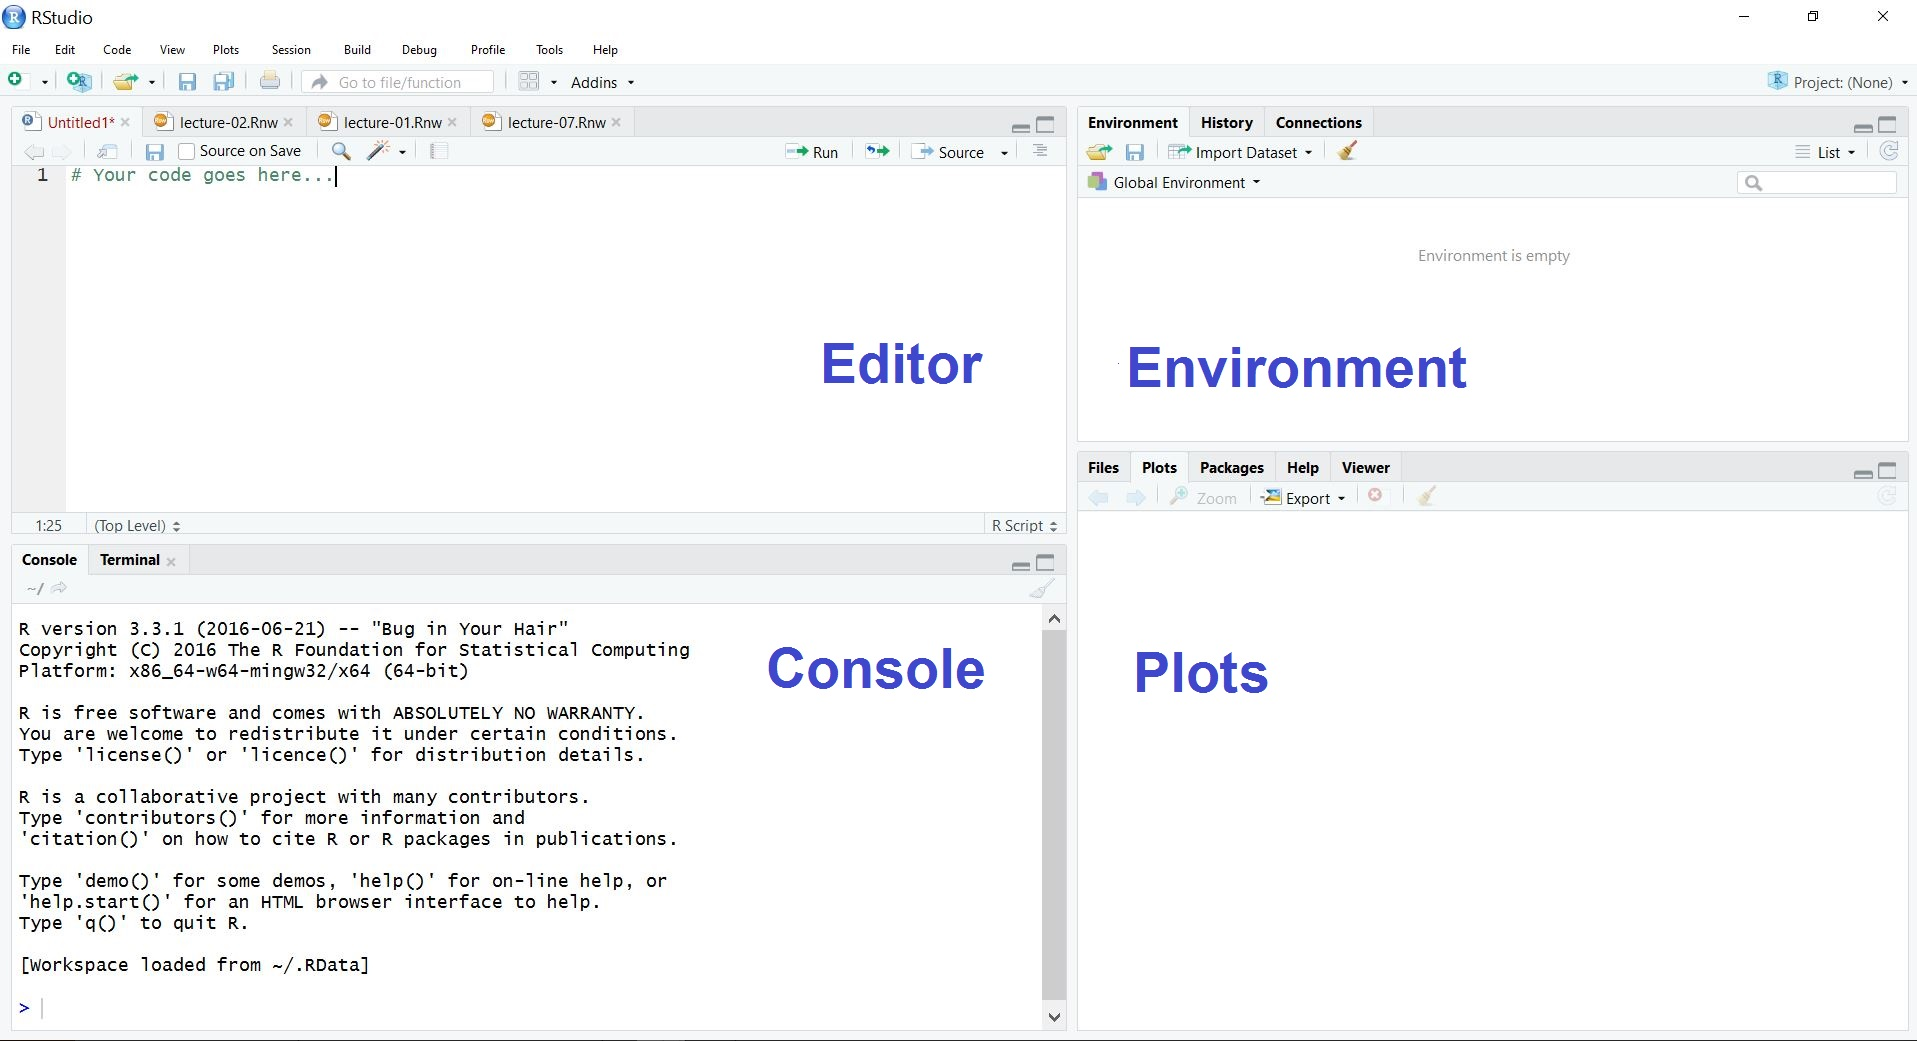
\includegraphics[width=4in]{RStudio}
      \end{center} 
    \end{frame}

    
    
    \begin{frame}{RStudio Layout}
    \fontsize{10}{10}\selectfont
      \begin{itemize}
        \item \alert{Console:} This is where calculations/code are passed to R and results are observed. \pause
        \item \alert{Editor:} It is not practical to write long calculations/code in console. We write them in the editor, and "Run" to pass to the console. \pause
        \item \alert{Environment:} All data sets/variables we define can be found here. \pause
        \item \alert{Plots:} When we plot things, they will first appear here.
      \end{itemize} 
    \end{frame}
    
    
    
    
    \begin{frame}{Let's get started...}
    \fontsize{10}{10}\selectfont
    Assume you want to calculate your course grade.
    
      \begin{table}[!b]
        {\carlitoTLF % Use monospaced lining figures
        \begin{tabularx}{\textwidth}{ccc}
           
           Assignment & Weight  & Grade \\ 
          \toprule
            Class participation & 5\%	&	91  \\
            Reading assignments & 5\%	&	95  \\
            Homework    & 15\%	&	 86 \\
            Project     & 15\%	&	 83 \\
            Midterm 1   & 20\%	&	 88 \\
            Midterm 2   & 20\%	&	 76 \\
            Final exam  & 20\%	&	 84 \\
        \end{tabularx}}
        
      \end{table} 
    \end{frame}


    \begin{frame}[fragile]{Using the console}
      First try this in console.
\begin{knitrout}
\definecolor{shadecolor}{rgb}{0.137, 0.137, 0.137}\begin{kframe}
\begin{alltt}
\hlstd{> }  \hlnum{0.05}\hlopt{*}\hlnum{91}\hlopt{+}\hlnum{0.05}\hlopt{*}\hlnum{95}\hlopt{+}\hlnum{0.15}\hlopt{*}\hlnum{86}\hlopt{+}\hlnum{0.15}\hlopt{*}\hlnum{83}\hlopt{+}\hlnum{0.2}\hlopt{*}\hlnum{88}\hlopt{+}\hlnum{0.2}\hlopt{*}\hlnum{76}\hlopt{+}\hlnum{0.2}\hlopt{*}\hlnum{84}
\end{alltt}
\begin{verbatim}
[1] 84.25
\end{verbatim}
\end{kframe}
\end{knitrout}
      \pause
      It makes sense to save the result to a variable to be able to use later.
\begin{knitrout}
\definecolor{shadecolor}{rgb}{0.137, 0.137, 0.137}\begin{kframe}
\begin{alltt}
\hlstd{> }  \hlstd{my371} \hlkwb{<-} \hlnum{0.05}\hlopt{*}\hlnum{91}\hlopt{+}\hlnum{0.05}\hlopt{*}\hlnum{95}\hlopt{+}\hlnum{0.15}\hlopt{*}\hlnum{86}\hlopt{+}\hlnum{0.15}\hlopt{*}\hlnum{83}\hlopt{+}\hlnum{0.2}\hlopt{*}\hlnum{88}\hlopt{+}\hlnum{0.2}\hlopt{*}\hlnum{76}\hlopt{+}\hlnum{0.2}\hlopt{*}\hlnum{84}
\end{alltt}
\end{kframe}
\end{knitrout}
    \end{frame}



    \begin{frame}[fragile]{Using the editor}
      \fontsize{10}{10}\selectfont
      It much convenient to do the calculations/coding in the editor and then "run" them. \pause
      
      Working with vectors is also common, which are simply data containers.

\begin{knitrout}
\definecolor{shadecolor}{rgb}{0.137, 0.137, 0.137}\begin{kframe}
\begin{alltt}
\hlstd{> }  \hlcom{# This is the same calculation, using vectors.}
\hlstd{> }  \hlstd{weights} \hlkwb{<-} \hlkwd{c}\hlstd{(}\hlnum{0.05}\hlstd{,} \hlnum{0.05}\hlstd{,} \hlnum{0.15}\hlstd{,} \hlnum{0.15}\hlstd{,} \hlnum{0.2}\hlstd{,} \hlnum{0.2}\hlstd{,} \hlnum{0.2}\hlstd{)}
\hlstd{> }  \hlstd{grades} \hlkwb{<-} \hlkwd{c}\hlstd{(}\hlnum{91}\hlstd{,} \hlnum{95}\hlstd{,} \hlnum{86}\hlstd{,} \hlnum{83}\hlstd{,} \hlnum{88}\hlstd{,} \hlnum{76}\hlstd{,} \hlnum{84}\hlstd{)}
\hlstd{> }  \hlstd{weighted_grades} \hlkwb{<-} \hlstd{weights}\hlopt{*}\hlstd{grades}
\hlstd{> }  \hlstd{my371} \hlkwb{<-} \hlkwd{sum}\hlstd{(weighted_grades)}
\end{alltt}
\end{kframe}
\end{knitrout}
      The multiplication is element-wise. \pause
      
      ``sum'' is a predefined function in R, which sums all the elements in a vector.
  
      \note{Discuss why it makes sense to vectorize and save in variables. We can, for example, use weights in multiple places.}

    \end{frame}
    
    
    
    \begin{frame}[fragile]{Working with tabular data}
      \fontsize{10}{10}\selectfont
      Many data sets we will work with are in tabular format, saved in .csv files. \pause
      
      Let's analyze the passenger data from the Titanic disaster.
      \begin{center}
        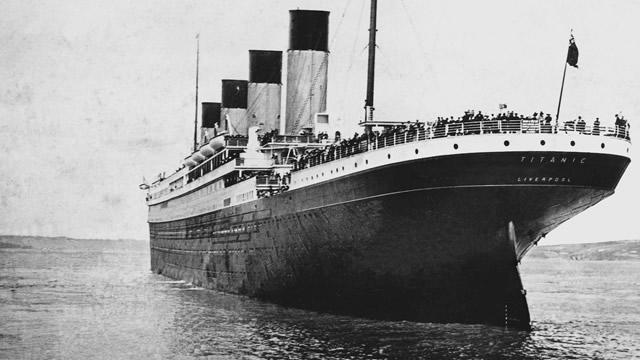
\includegraphics[width=4in]{titanic}
      \end{center} 
    
    
    \end{frame}
    
    
    
    \begin{frame}[fragile]{Working with tabular data}
      \fontsize{10}{10}\selectfont
      In order to see the table, use "View(titanic)". \pause
      
      \bigskip
      
      "\$" sign is used to refer to a particular column in the data, such as "titanic\$Name".   \pause
      
      \bigskip
      
      To access to an element in a particular position, e.g., row 1, column 4, use "titanic[1,4]".
      
    
    \end{frame}
    
    
    \begin{frame}[fragile]{Exploring Categorical Variables}  
      \fontsize{10}{10}\selectfont
      The dataset has both quantitative and categorical data. \pause
      
      Let's explore the categorical variables through some frequency tables. \pause
      
      Below is the number of passengers in each class.
      
\begin{knitrout}
\definecolor{shadecolor}{rgb}{0.137, 0.137, 0.137}\begin{kframe}
\begin{alltt}
\hlstd{> }  \hlkwd{table}\hlstd{(titanic}\hlopt{$}\hlstd{PClass)}
\end{alltt}
\begin{verbatim}

1st 2nd 3rd 
323 279 711 
\end{verbatim}
\end{kframe}
\end{knitrout}
      
    \end{frame}  
    
    
    \begin{frame}[fragile]{Exploring Categorical Variables} 
      \fontsize{10}{10}\selectfont
      What is more interesting is how many people survived in each passenger class. \pause
\begin{knitrout}
\definecolor{shadecolor}{rgb}{0.137, 0.137, 0.137}\begin{kframe}
\begin{alltt}
\hlstd{> }  \hlstd{class_survival} \hlkwb{<-} \hlkwd{table}\hlstd{(titanic}\hlopt{$}\hlstd{Survived, titanic}\hlopt{$}\hlstd{PClass)}
\hlstd{> }  \hlstd{class_survival}
\end{alltt}
\begin{verbatim}
     
      1st 2nd 3rd
  No  130 160 573
  Yes 193 119 138
\end{verbatim}
\end{kframe}
\end{knitrout}
    \end{frame}
    
    
    \begin{frame}[fragile]{Exploring Categorical Variables}
      \fontsize{10}{10}\selectfont
      To get a better sense of the data, let's calculate the survival percentage for each passenger class.
\begin{knitrout}
\definecolor{shadecolor}{rgb}{0.137, 0.137, 0.137}\begin{kframe}
\begin{alltt}
\hlstd{> }  \hlkwd{prop.table}\hlstd{(class_survival,}\hlnum{2}\hlstd{)}
\end{alltt}
\begin{verbatim}
     
            1st       2nd       3rd
  No  0.4024768 0.5734767 0.8059072
  Yes 0.5975232 0.4265233 0.1940928
\end{verbatim}
\end{kframe}
\end{knitrout}
      \pause
      It looks like one's chance of survival highly depended on his/her passenger class...
    \end{frame}
    
    
    
    \begin{frame}[fragile]{Slicing the data}
      \fontsize{10}{10}\selectfont
      One very common operation is slicing the data, i.e., selecting the portion that satisfy certain conditions. \pause
      
      \bigskip
      For example, we can select the rows that belong to female passenger data.
\begin{knitrout}
\definecolor{shadecolor}{rgb}{0.137, 0.137, 0.137}\begin{kframe}
\begin{alltt}
\hlstd{> }   \hlstd{female_psg} \hlkwb{<-} \hlstd{titanic[titanic}\hlopt{$}\hlstd{Sex}\hlopt{==}\hlstr{'female'}\hlstd{,]}
\end{alltt}
\end{kframe}
\end{knitrout}
      \pause
      
      This means: in the titanic dataset, select rows where the "Sex" is "female", select all columns, and save the resulting table to "female\_psg" variable.

    \end{frame}
    
    
    
    
    \begin{frame}[fragile]{Slicing the data}
      \fontsize{10}{10}\selectfont
      We can create more complex conditions.
      
\begin{knitrout}
\definecolor{shadecolor}{rgb}{0.137, 0.137, 0.137}\begin{kframe}
\begin{alltt}
\hlstd{> }  \hlstd{female_psg_1st} \hlkwb{<-} \hlstd{titanic[(titanic}\hlopt{$}\hlstd{Sex}\hlopt{==}\hlstr{'female'}\hlstd{)} \hlopt{&}
\hlstd{+ }                                \hlstd{(titanic}\hlopt{$}\hlstd{PClass}\hlopt{==}\hlstr{'1st'}\hlstd{),]}
\end{alltt}
\end{kframe}
\end{knitrout}
    
    \end{frame}
    
    
    
    
    \begin{frame}[fragile]{Cleaning the data}
      \fontsize{10}{10}\selectfont
      If you want to analyze the "Age" data, you will realize rows with "NA", meaning Not Available. \pause
      
      \bigskip
      Let's select rows where we have age data available.
      
\begin{knitrout}
\definecolor{shadecolor}{rgb}{0.137, 0.137, 0.137}\begin{kframe}
\begin{alltt}
\hlstd{> }  \hlstd{titanic_age} \hlkwb{<-} \hlstd{titanic[}\hlopt{!}\hlkwd{is.na}\hlstd{(titanic}\hlopt{$}\hlstd{Age),]}
\end{alltt}
\end{kframe}
\end{knitrout}
      \pause
      This selects rows where the Age value is not "NA".
      
    \end{frame}  
    
    
    
    \begin{frame}[fragile]{Exploring quantitative data}
      \fontsize{10}{10}\selectfont
      Let's look into age distribution of the passengers.
      
\begin{knitrout}
\definecolor{shadecolor}{rgb}{0.137, 0.137, 0.137}\begin{kframe}
\begin{alltt}
\hlstd{> }\hlkwd{hist}\hlstd{(titanic_age}\hlopt{$}\hlstd{Age,} \hlkwc{col}\hlstd{=}\hlstr{'green'}\hlstd{,} \hlkwc{main}\hlstd{=}\hlstr{''}\hlstd{)}
\end{alltt}
\end{kframe}
\input{/tmp/figures/unnamed-chunk-12-1.tikz}

\end{knitrout}
      
    \end{frame}
    
    
        \begin{frame}[fragile]{Exploring quantitative data}
      \fontsize{10}{10}\selectfont
      Another way to look into it, by using a boxplot and compare between passenger classes.
      
\begin{knitrout}
\definecolor{shadecolor}{rgb}{0.137, 0.137, 0.137}\begin{kframe}
\begin{alltt}
\hlstd{> }\hlkwd{boxplot}\hlstd{(Age} \hlopt{~} \hlstd{PClass,} \hlkwc{data}\hlstd{=titanic,} \hlkwc{col}\hlstd{=}\hlstr{'green'}\hlstd{,} \hlkwc{main}\hlstd{=}\hlstr{''}\hlstd{)}
\end{alltt}
\end{kframe}
\input{/tmp/figures/unnamed-chunk-13-1.tikz}

\end{knitrout}
      
    \end{frame}
    
    
    

  \end{darkframes}

\end{document}

